\documentclass[journal]{IEEEtran} % use the `journal` option for ITherm conference style
\IEEEoverridecommandlockouts
% The preceding line is only needed to identify funding in the first footnote. If that is unneeded, please comment it out.
\usepackage{cite}
\usepackage{amsmath,amssymb,amsfonts}
\usepackage{algorithmic}
\usepackage{graphicx}
\usepackage{textcomp}
\usepackage{xcolor}
\def\BibTeX{{\rm B\kern-.05em{\sc i\kern-.025em b}\kern-.08em
    T\kern-.1667em\lower.7ex\hbox{E}\kern-.125emX}}
\begin{document}

\title{Statistical Authorship Attribution And Analysis Of Agatha
Christie’s Works
% delete or comment-out the following line before submission
% {\footnotesize \textsuperscript{*}Note: Sub-titles are not captured in Xplore and should not be used}
% \thanks{Professor Begoli and our TA Gomathi}
}

\author{%%%% author names
    \IEEEauthorblockN{Adam Ryan McDaniel}% first author
    , \IEEEauthorblockN{Ahmad Amirivojdan}
    , \IEEEauthorblockN{Vincent Gregory Broda}
    , \IEEEauthorblockN{Mohamed Shatarah}
    % duplicate the line above as many times as needed to list all authors
    \\%%%% author affiliations
    \IEEEauthorblockA{\textit{EECS UTK, Knoxville, Tennessee}}\\% first affiliation
    % duplicate the line above as many times as needed to list all affiliations
    %%%% corresponding author contact details
    \IEEEauthorblockA{amcdan23@vols.utk.edu}
    , \IEEEauthorblockA{aamirivo@vols.utk.edu}
    , \IEEEauthorblockA{vbroda@vols.utk.edu}
    , \IEEEauthorblockA{mshatara@vols.utk.edu}
}

\maketitle

\begin{abstract}
    This document is our report for Project \#1 of COSC 524, Natural Language Processing. It outlines our statistics based approach to performing authorship attribution to given works, specifically targeting Agatha Christie.
\end{abstract}

\begin{IEEEkeywords}
    statistics, NLP, tokenization, supervised ML, unsupervised ML
\end{IEEEkeywords}

\section{Introduction}
Authorship attribution is a crucial task in the field of natural language processing, where the author of a given text is determined based on linguistic and stylistic patterns \cite{misini2022}. This project focuses on developing an authorship analysis model specifically for Agatha Christie, a famous crime and mystery novelist. The primary purpose of this project is to construct a statistical model capable of attributing authorship to Agatha Christie among a set of other arbitrary authors. The dataset used for training included 4 other authors: Maurice Leblanc, G. K. Chesterton, Lewis Carroll, and Herman Melville. The texts were sourced from Project Gutenberg, providing a diverse dataset for analysis. By analyzing stylistic and linguistic features extracted from the texts, the aim is to capture the unique aspects of Christie's writing style. Machine learning techniques such as logistic regression and clustering algorithms are employed to differentiate her works from others.

\section{Methodology}
A total of 64 novels from Project Gutenberg were collected to form the dataset. This included 12 novels by Agatha Christie and 52 novels by other authors: Maurice Leblanc, G.K. Chesterton, Lewis Carroll, and Herman Melville. Table \ref{tab1} shows the novel counts for each author. These authors were chosen due to similarities in genre and style, providing a challenging dataset for authorship attribution. To better handle lengthy texts, the novels were split into chapters, and further into 100-sentence-long chunks. This segmentation improved the accuracy of the model by allowing finer feature analysis.

\subsection{Data Preprocessing}  
To prepare the texts for feature extraction, standard text-cleaning steps were performed. This included:
\begin{enumerate}
    \item \textbf{Tokenization:} Splitting text into sentences and words.
    \item \textbf{Normalization:} Lowercasing and splitting punctuation into separate tokens to standardize text.
    \item \textbf{Chunking:} Splitting novels into 100-sentence sections to handle lengthy texts effectively. To predict the author of a text, a majority vote of predictions for each chunk in the text is taken.
\end{enumerate}

\subsection{Feature Extraction}  
A variety of textual and stylometric features were extracted for each text or partial chunk of a whole text:

\begin{itemize}
    \item Textual Features
    \begin{enumerate}
        \item \textbf{N-grams:} Unigrams, bigrams, and trigrams captured frequently used word sequences, helping to identify patterns in word choice and syntax. \cite{misini2022}
        \item \textbf{TF-IDF}: Terms were weighted by their importance across all novels to prioritize unique vocabulary for each author. \cite{manning2008}
        $$\text{TF-IDF}(t, d, D) = \text{TF}(t, d) \times \text{IDF}(t, D)$$
        $$\text{TF}(t, d) = \frac{f_{t,d}}{\sum_{t' \in d} f_{t',d}}$$
        $$\text{IDF}(t, D) = \log\left(\frac{N}{| \{d \in D : t \in d \} |}\right)$$
    \end{enumerate}
    \item Stylometric Features
    \begin{enumerate}
        \item \textbf{Sentence Length Variation:} The variance of all the sentence lengths in the text, in terms of number of tokens. \cite{roelleke}
        \item \textbf{Word Length Variation:} The variance of all the word lengths in the text, in terms of number of characters. \cite{misini2022}
        \item \textbf{Average Sentence Length:} The average number of tokens in a sentence.
        \item \textbf{Average Word Length:} The average number of characters in a word.
        \item \textbf{Punctuation Frequency:} The frequency of punctuation marks in the text: commas, periods, exclamation marks, and question marks.
        \item \textbf{Lexical Diversity:} The ratio of unique words to total words in the text.
        \item \textbf{Adverb Frequency:} The frequency of adverbs in the text.
        \item \textbf{Contraction Density:} The ratio of contractions to total words in the text.
        \item \textbf{Pronoun Density:} The ratio of pronouns to total words in the text.
        \item \textbf{Quote Density:} The concentration of quotes in the text.
    \end{enumerate}
    \item Advanced Features
    \begin{enumerate}
        \item \textbf{Passive Voice Frequency:} The frequency of passive voice constructions in the text.
        \item \textbf{Estimated Grade Level:} A number representing the estimated grade level required to understand the text. This is a commonly used readability metric called the Flesch-Kincaid Grade Level \cite{flesch1975}.
        $$
        \text{g} = 0.39 \left(\frac{\text{Words}}{\text{Sentences}}\right) + 11.8 \left(\frac{\text{Syllables}}{\text{Words}}\right) - 15.59
        $$
    \end{enumerate}
\end{itemize}

These features were chosen to reflect both the content and the style of the authors, aiming to capture subtle differences in writing habits.

\subsection{Experiments}

The corpus is composed of the following works:

% Agatha Christie (12 novels)
% Maurice Leblanc (14 novels)
% GK Chesterton (21 novels)
% Lewis Carroll (3 novels)
% Herman Melville (4 novels)
\begin{table}[htbp]
    \begin{center}
        \begin{tabular}{|c|c|}
            \hline
            \textbf{Author} & \textbf{Number of Complete Novels} \\
            \hline
            \hline
            Agatha Christie & 12 \\
            \hline
            Maurice Leblanc & 17 \\
            \hline
            G.K. Chesterton & 26 \\
            \hline
            Lewis Carroll & 4 \\
            \hline
            Herman Melville & 5 \\
            \hline
        \end{tabular}
        \label{tab1}
    \end{center}
    \caption{Number of Works by Author}
\end{table}

The dataset was split into training and testing sets, with 80\% of the data used for training and 20\% for testing.
The experiments were executed using Python in a Jupyter Notebook, with a Python 3.12 environment. The machine used has an M3-Max CPU with 16 single-threaded cores and 128 gigabytes of unified memory. The following experiments were conducted:

\subsubsection{Variance Analysis Experiment}

Each feature was analyzed for variance across the authors to determine its effectiveness in distinguishing between them. The distribution of different features were graphed in 3-dimensions to visualize the clusters and discriminatory power of each dimension.

\subsubsection{K-Means Clustering Experiment}

K-means clustering was performed on the extracted features to investigate whether the texts naturally group according to authorship without using labels, as clustering methods have proven effective in stylistic analysis. \cite{roelleke} Then, the greedy register allocation algorithm was repurposed to assign clusters to their appropriate authors. The model was trained on the entire novels and evaluated on the validation set.

\subsubsection{Logistic Regression Binary Classification Experiment}

The first supervised model was a logistic regression model, using TF-IDF to distinguish texts authored by Agatha Christie and those by other authors.
The model was also trained on the feature vectors extracted, and then evaluated on the validation set as well.

\subsubsection{Support Vector Machine Multiclass Classification Experiment}

The second supervised model was an extended iteration of the logistic regression model, using a support vector machine (SVM) instead to classify texts into one of the five authors. The model was trained only on sentence chunks in order to identify authors, and was then tested against the validation set.

\subsubsection{Binary Decision Tree Classification Experiment}

The final supervised model was a decision tree classifier, using the same features as the logistic regression model. The model was trained only on the chunks of sentences, and then additionally evaluated on the validation set.

\section{Results}

\subsection{Variance Analysis Experiment}

The variance of each feature from author to author is plotted in a bar-chart in Figure \ref{vary1}. Few features have massive variance, while the majority of features vary only slightly between authors. The most important features were determined to be average sentence length, sentence length variation, and average word length.

\begin{figure}
    \caption{Variance of Features Across Authors}
    \begin{center}
    \centerline{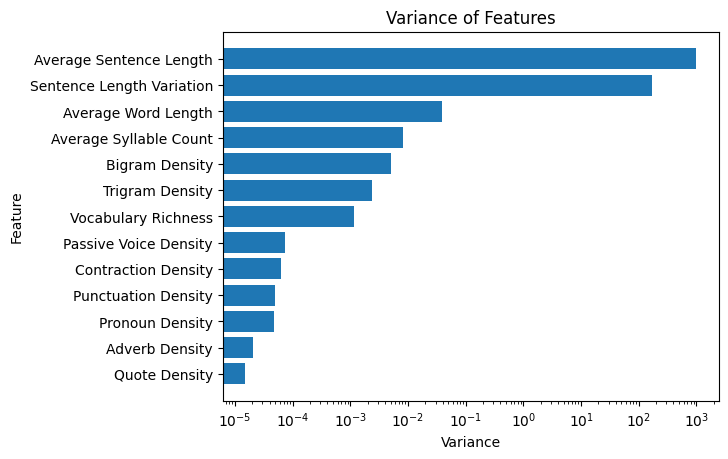
\includegraphics[width=0.48\textwidth]{./vary1.png}}
    \end{center}
    \centering
    \label{vary1}
\end{figure}

The three top features were plotted in 3D space to visualize the clusters formed by the authors. Figure \ref{vary2} shows the clusters formed by the authors in the feature space. There is usually a clear separation between authors, indicating that these metrics are useful for distinguishing between them.

\begin{figure}[h!]
    \caption{3D Plot of Top Features}
    \begin{center}
    \centerline{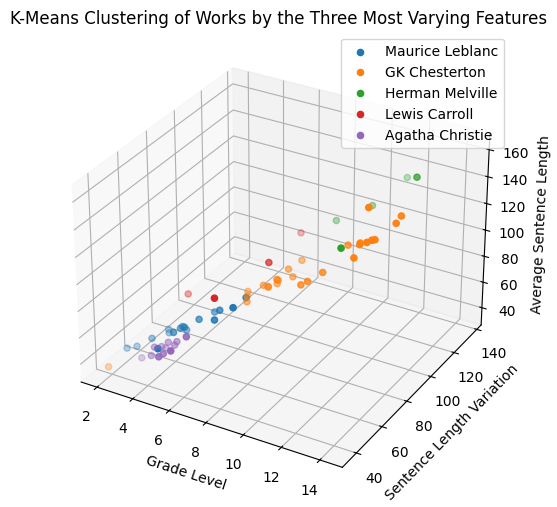
\includegraphics[width=0.35\textwidth]{./vary2.png}}
    \end{center}
    \centering
    \label{vary2}
\end{figure}

Next, the three median features were plotted in 3D space to visualize the clusters formed by the authors. Figure \ref{vary3} shows the same visualization as Figure \ref{vary2}, but with the median features instead of the top features. There is much less clear separation between these groups, showing that these features are less discriminative.

\begin{figure}
    \caption{3D Plot of Features With Median Importance}
    \begin{center}
    \centerline{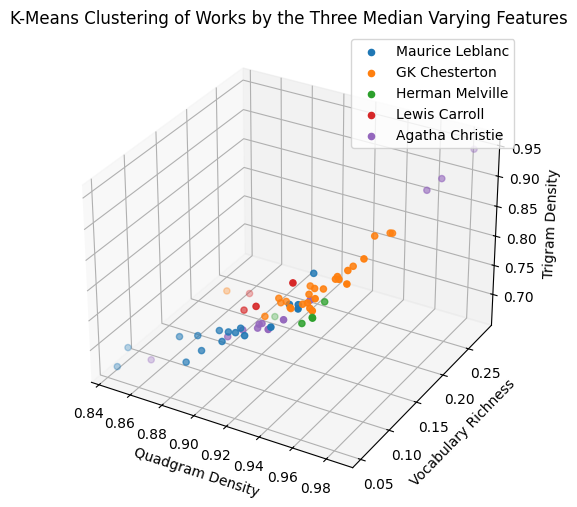
\includegraphics[width=0.45\textwidth]{./vary3.png}}
    \end{center}
    \centering
    \label{vary3}
\end{figure}

Finally, the lowest three important features were plotted. Figure \ref{vary4} shows the same visualization as Figure \ref{vary2}, but with the lowest features instead of the top features. There is significant overlap between the groups, showing that these features are not useful at all for distinguishing between authors.

\begin{figure}[h!]
    \caption{3D Plot of Features With Lowest Importance}
    \begin{center}
    \centerline{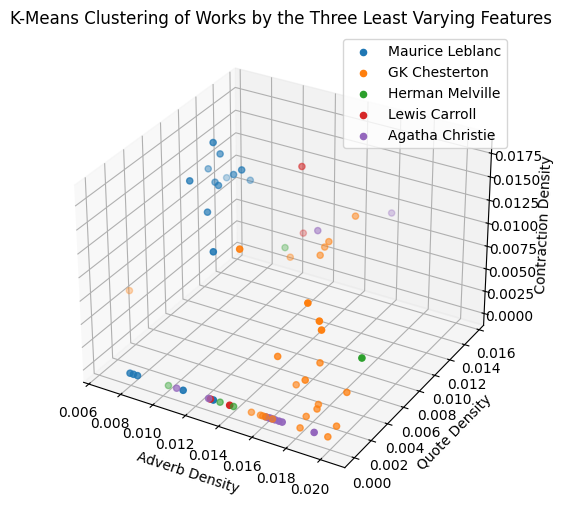
\includegraphics[width=0.35\textwidth]{./vary4.png}}
    \end{center}
    \centering
    \label{vary4}
\end{figure}

\subsection{K-Means Clustering Experiment}

The K-means clustering model was able to cluster the feature vectors into five distinct clusters, corresponding to the five authors, however the classification for many works were very confused. Figure \ref{kmeans} shows the confusion matrix of the clustering.
Agatha Christie's works were all correctly identified, but other authors were often misclassified. The overall accuracy across all works was 62.5\%. This approach was inefficient and did not yield satisfactory results.

\begin{figure}[h!]
    \caption{K-Means Clustering Results}
    \begin{center}
    \centerline{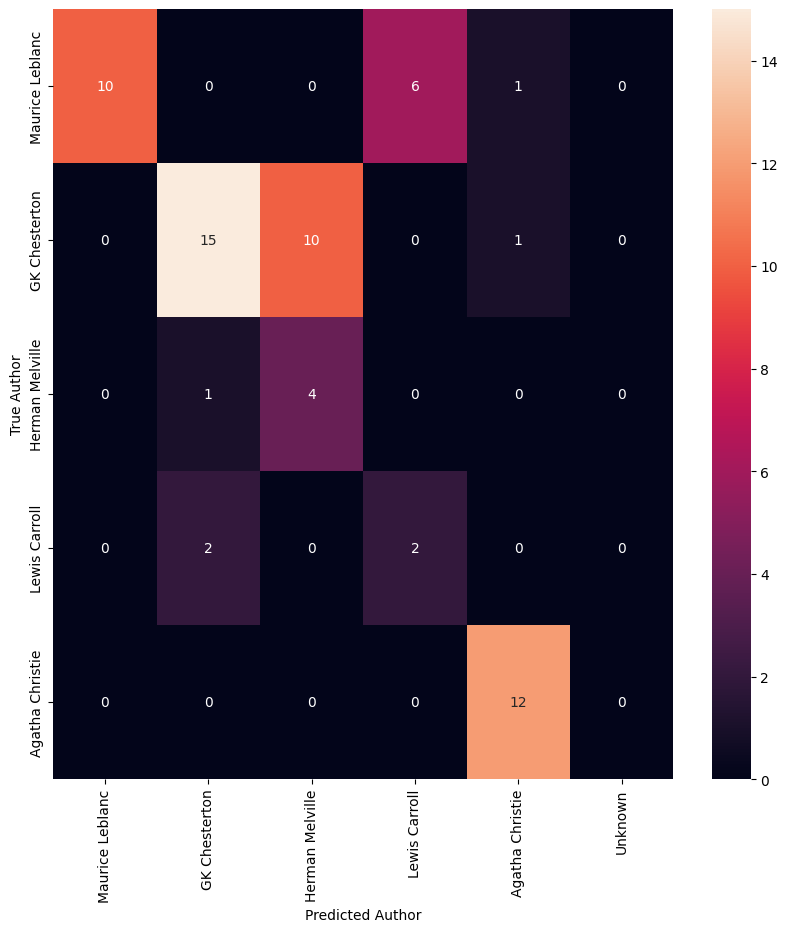
\includegraphics[width=0.35\textwidth]{./kmeans.png}}
    \end{center}
    \centering
    \label{kmeans}
\end{figure}

\subsection{Logistic Regression Binary Classification Experiment}

Classifying each text using TF-IDF and logistic regression yielded an accuracy of 100\% for the custom validation dataset, distinguishing authors: the model was able to accurately predict whether Agatha Christie was the author of all the texts. Figure \ref{logreg} shows the confusion matrix of the logistic regression model.

This method was successful at identifying texts, but the final, superior model was the decision tree based model for high explainability and reproducilbility while maintaining accuracy.

\begin{figure}[h!]
    \caption{Logistic Regression Binary Classification Results}
    \begin{center}
    \centerline{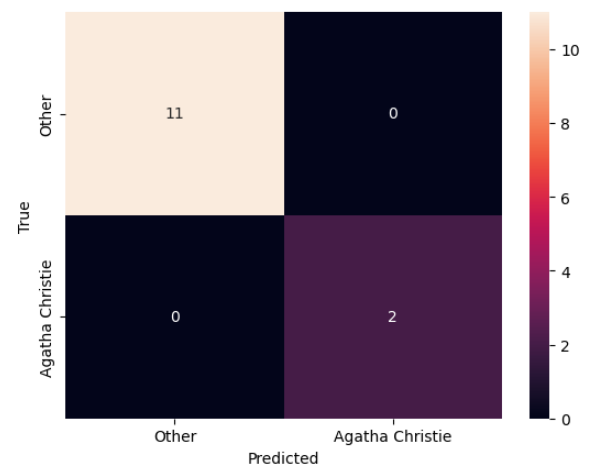
\includegraphics[width=0.4\textwidth]{./logreg.png}}
    \end{center}
    \centering
    \label{logreg}
\end{figure}

\subsection{Support Vector Machine Multiclass Classification Experiment}

The SVM model was trained only on sentence chunks and evaluated on the validation set. The model achieved an accuracy of 99\% on the validation set, only misclassifiying 13 chunks out of over 1,000 total chunks. Figure \ref{svm} shows the confusion matrix of the SVM model.

\begin{figure}
    \caption{SVM Multiclass Classification Results}
    \begin{center}
    \centerline{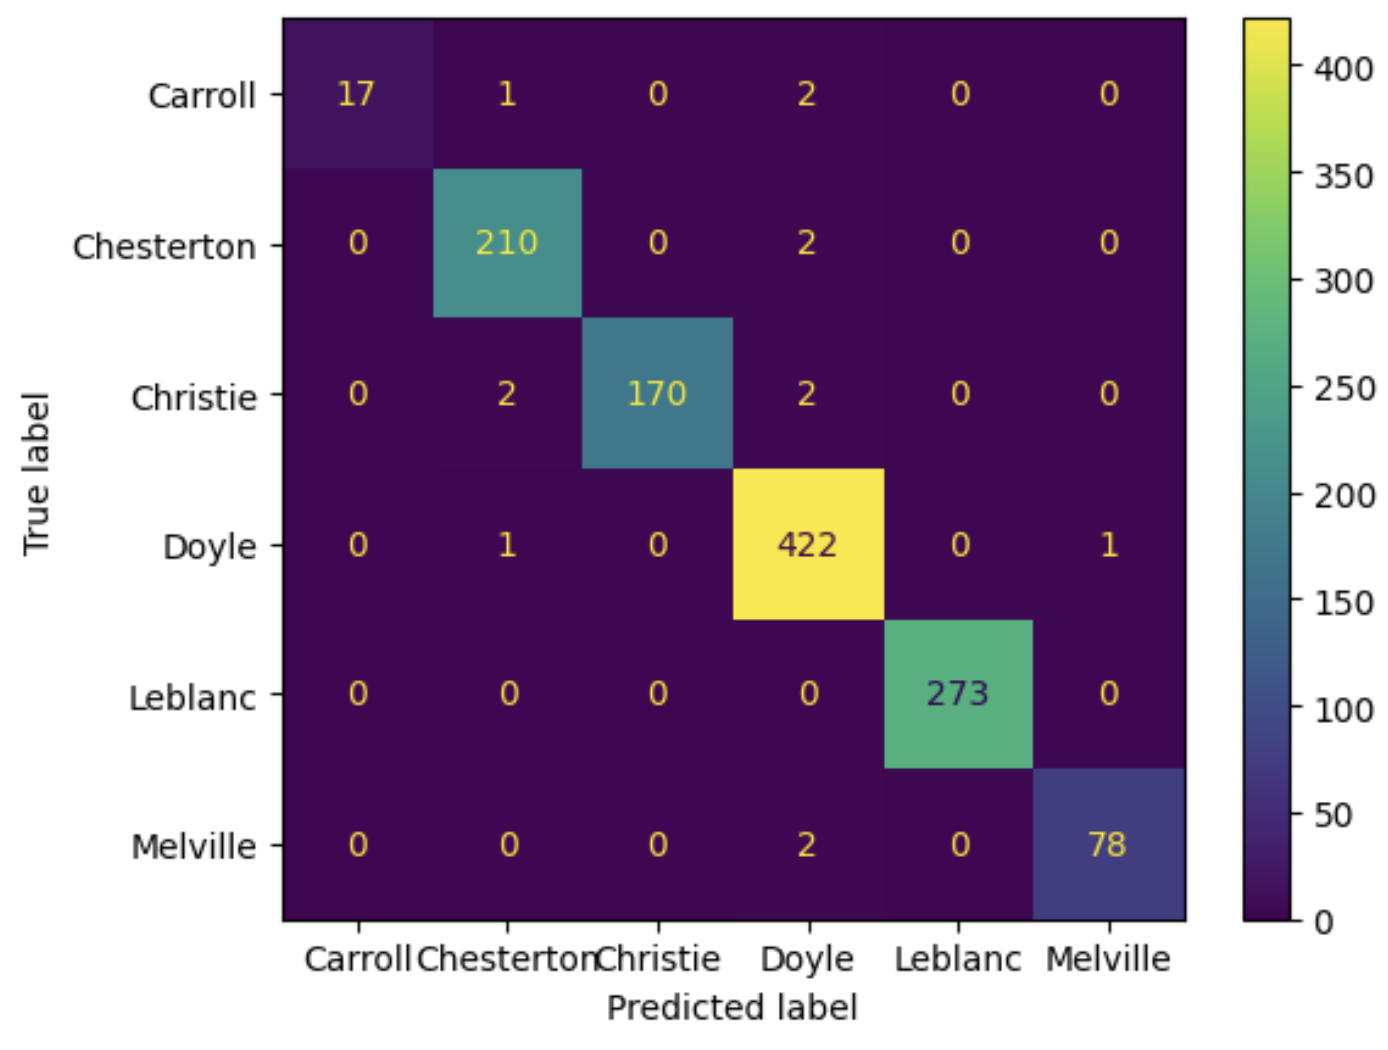
\includegraphics[width=0.4\textwidth]{./svm.png}}
    \end{center}
    \centering
    \label{svm}
\end{figure}

\subsection{Binary Decision Tree Classification Experiment}

The chunk approach was adapted to perform prediction for a whole text. The work is chunked into blocks of N sentence, featurized, and a majority vote is taken based on the predicted classification of each chunk.

\begin{figure}[h!]
    \caption{Decision Tree Binary Classification Results On Custom Validation Set}
    \begin{center}
    \centerline{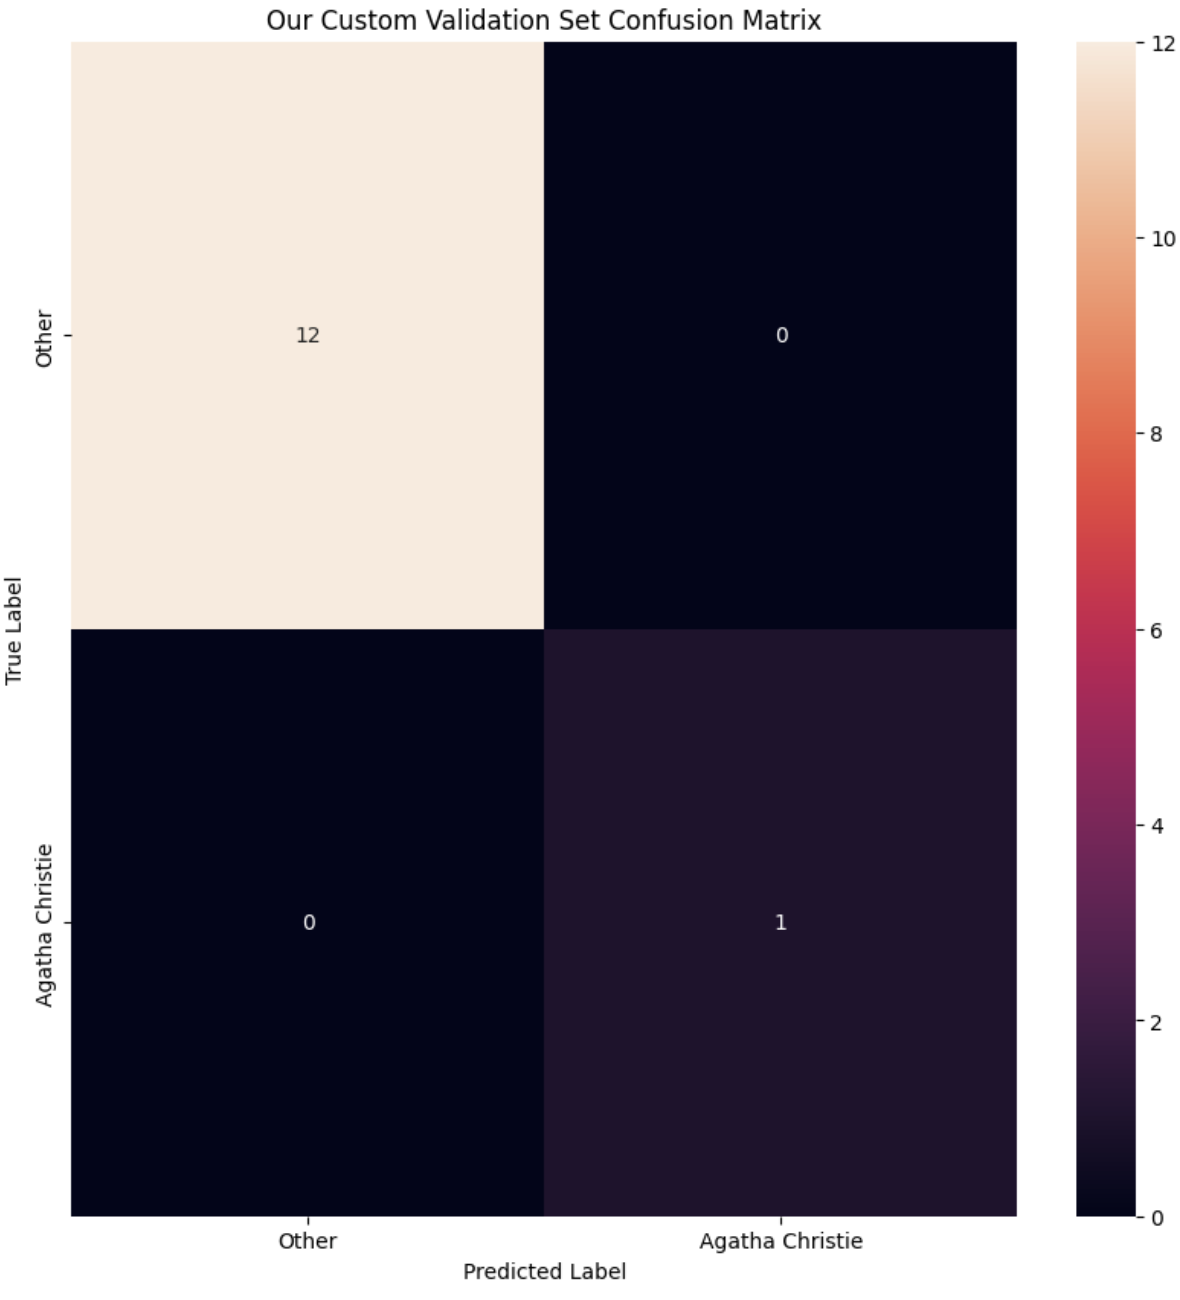
\includegraphics[width=0.4\textwidth]{./dt1.png}}
    \end{center}
    \centering
    \label{dt}
\end{figure}

The chunk size of 100 was found to be an ideal candidate for the chunk size: with larger chunk sizes, there are fewer sentences per chunk and their feature vectors aren't representative of the work's author. With chunks that are too small, the feature vectors are too noisy and don't represent the work's author, either. The decision tree model achieved an accuracy of 100\% on the validation set, with no misclassifications. Figure \ref{dt} shows the confusion matrix of the decision tree model on the custom validation dataset.
With the provided dataset from the class, the following confusion matrix was obtained for the decision tree model. The model achieved an accuracy of 100\% on the validation set, with no misclassifications. Figure \ref{dt2} shows the confusion matrix of the decision tree model on the provided dataset. This final model achieved 100\% accuracy on the custom validation dataset, and 83.33\% accuracy on the provided dataset.
This final model was chosen for its explainability and equally high accuracy.

\begin{figure}
    \caption{Decision Tree Binary Classification Results On Provided Validation Set}
    \begin{center}
    \centerline{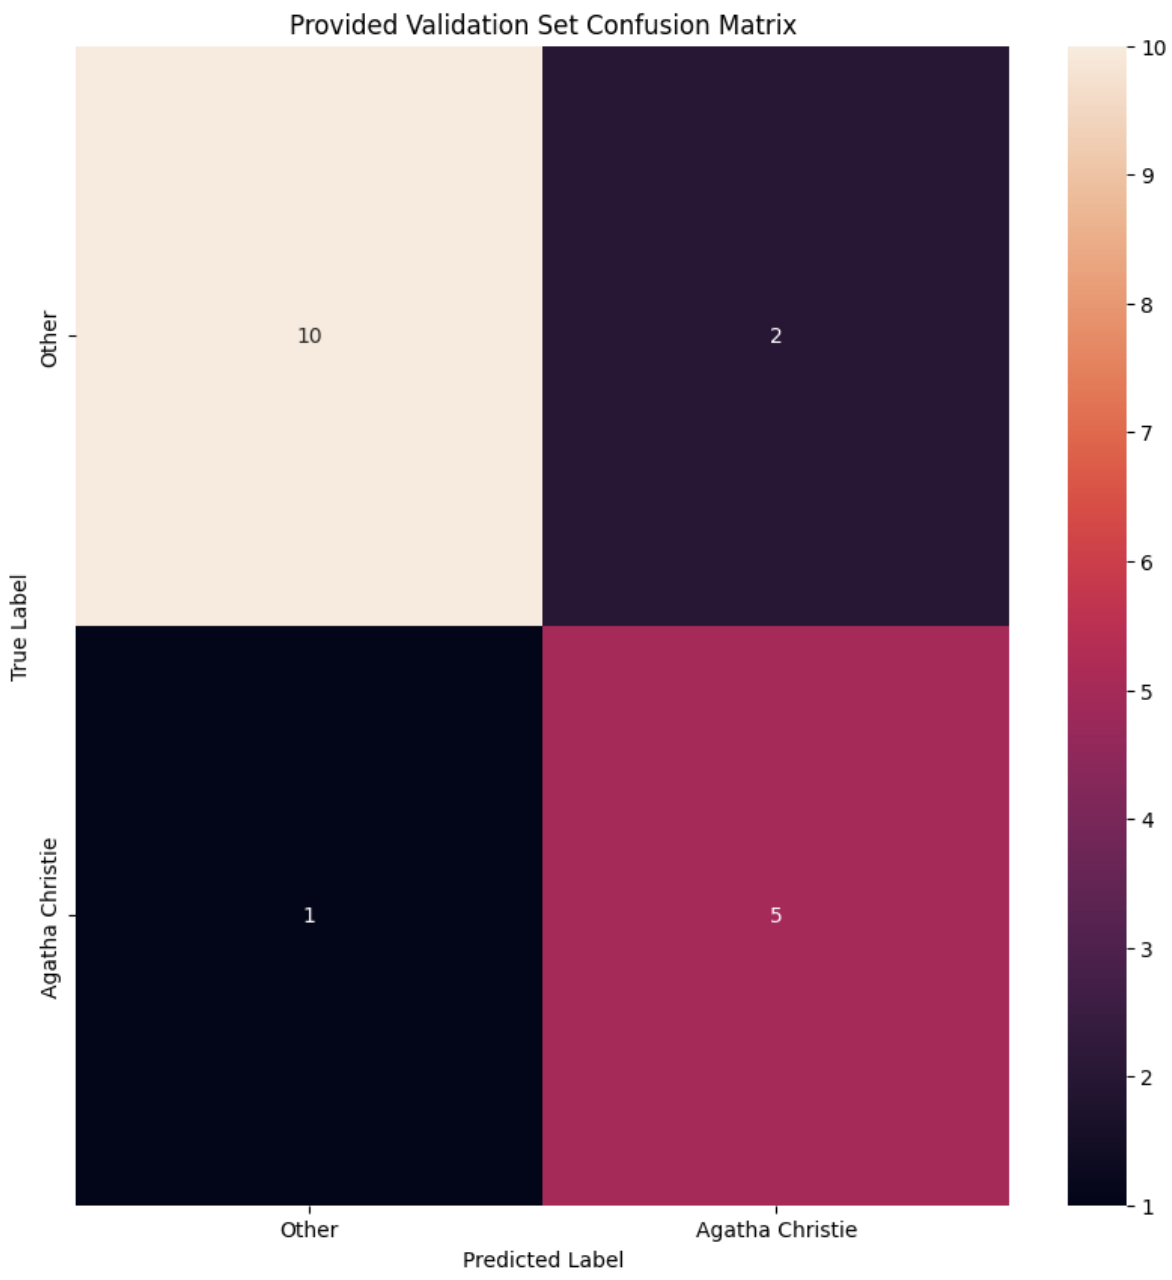
\includegraphics[width=0.4\textwidth]{./dt2.png}}
    \end{center}
    \centering
    \label{dt2}
\end{figure}

\begin{table}
    \begin{center}
        \begin{tabular}{|c|c|c|}
            \hline
            \textbf{Text} & \textbf{Predicted Author}  & \textbf{Actual Author} \\
            \hline
            \hline
            Text \#1 & \textcolor{red}{Not Agatha Christie} & Agatha Christie \\
            \hline
            Text \#2 & Agatha Christie & Agatha Christie \\
            \hline
            Text \#3 & Agatha Christie & Agatha Christie \\
            \hline
            Text \#4 & Agatha Christie & Agatha Christie \\
            \hline
            Text \#5 & Agatha Christie & Agatha Christie \\
            \hline
            Text \#6 & Agatha Christie & Agatha Christie \\
            \hline
            Text \#7 & Not Agatha Christie & Arthur Conan Doyle \\
            \hline
            Text \#8 & Not Agatha Christie & Arthur Conan Doyle \\
            \hline
            Text \#9 & Not Agatha Christie & Arthur Conan Doyle \\
            \hline
            Text \#10 & Not Agatha Christie & Arthur Conan Doyle \\
            \hline
            Text \#11 & \textcolor{red}{Agatha Christie} & Arthur Conan Doyle \\
            \hline
            Text \#12 & \textcolor{red}{Agatha Christie} & Arthur Conan Doyle \\
            \hline
            Text \#13 & Not Agatha Christie & G.K. Chesterton \\
            \hline
            Text \#14 & Not Agatha Christie & G.K. Chesterton \\
            \hline
            Text \#15 & Not Agatha Christie & G.K. Chesterton \\
            \hline
            Text \#16 & Not Agatha Christie & G.K. Chesterton \\
            \hline
            Text \#17 & Not Agatha Christie & G.K. Chesterton \\
            \hline
            Text \#18 & Not Agatha Christie & G.K. Chesterton \\
            \hline
        \end{tabular}
        \label{tab2}
    \end{center}
    \caption{Predicted Authorship Attribution Of Agatha Christie On Provided Dataset}
\end{table}

\section{Conclusion}

Several key features that distinguish Agatha Christie's writing style from other authors. Average sentence length, sentence length variation, and average word length are the most important features for prediction.

Our experiments demonstrate that supervised machine learning models, particularly decision tree and logistic regression models with TF-IDF features, are highly effective for authorship attribution in this context. The perfect accuracy on the custom validation set, and the high accuracy on the provided set, indicates that Agatha Christie's writing style is distinctly different from the other authors in the dataset.

It was revealed that unsupervised clustering may not be ideal for authorship attribution, as it yields lower precision and more confusion between authors.
While still lower in accuracy, though, unsupervised clustering results still showed that stylometric features carry authorial signals.

The decision tree model was demonstrated to be the most useful while maintaining effectiveness and interpretability. The method of featurizing N-sentence chunks of text with a majority vote proved to be the most effective method for authorship attribution.

The final model achieved 100\% accuracy on the custom validation dataset, and 83.33\% accuracy on the provided dataset. The model was able to accurately predict the author of Agatha Christie's works, and was able to distinguish her works from those of other authors. 

In conclusion, this work successfully presents an explainable, reasonably accurate, and reproducible decision tree model for authorship attribution of Agatha Christie's novels.

% Number equations consecutively. To make your
% equations more compact, you may use the solidus (~/~), the exp function, or
% appropriate exponents. Italicize Roman symbols for quantities and variables,
% but not Greek symbols. Use a long dash rather than a hyphen for a minus
% sign. Punctuate equations with commas or periods when they are part of a
% sentence, as in:
% \begin{equation}
%     a+b=\gamma\label{eq}
% \end{equation}

% Be sure that the
% symbols in your equation have been defined before or immediately following
% the equation. Use ``\eqref{eq}'', not ``Eq.~\eqref{eq}'' or ``equation \eqref{eq}'', except at
% the beginning of a sentence: ``Equation \eqref{eq} is . . .''

% \subsection{\LaTeX-Specific Advice}

% Please use ``soft'' (e.g., \verb|\eqref{Eq}|) cross references instead
% of ``hard'' references (e.g., \verb|(1)|). That will make it possible
% to combine sections, add equations, or change the order of figures or
% citations without having to go through the file line by line.

% Please don't use the \verb|{eqnarray}| equation environment. Use
% \verb|{align}| or \verb|{IEEEeqnarray}| instead. The \verb|{eqnarray}|
% environment leaves unsightly spaces around relation symbols.

% Please note that the \verb|{subequations}| environment in {\LaTeX}
% will increment the main equation counter even when there are no
% equation numbers displayed. If you forget that, you might write an
% article in which the equation numbers skip from (17) to (20), causing
% the copy editors to wonder if you've discovered a new method of
% counting.

%     {\BibTeX} does not work by magic. It doesn't get the bibliographic
% data from thin air but from .bib files. If you use {\BibTeX} to produce a
% bibliography you must send the .bib files.

%     {\LaTeX} can't read your mind. If you assign the same label to a
% subsubsection and a table, you might find that Table I has been cross
% referenced as Table IV-B3.

% {\LaTeX} does not have precognitive abilities. If you put a
% \verb|\label| command before the command that updates the counter it's
% supposed to be using, the label will pick up the last counter to be
% cross referenced instead. In particular, a \verb|\label| command
% should not go before the caption of a figure or a table.

% Do not use \verb|\nonumber| inside the \verb|{array}| environment. It
% will not stop equation numbers inside \verb|{array}| (there won't be
% any anyway) and it might stop a wanted equation number in the
% surrounding equation.

% \subsection{Some Common Mistakes}\label{SCM}
% \begin{itemize}
%     \item The word ``data'' is plural, not singular.
%     \item The subscript for the permeability of vacuum $\mu_{0}$, and other common scientific constants, is zero with subscript formatting, not a lowercase letter ``o''.
%     \item In American English, commas, semicolons, periods, question and exclamation marks are located within quotation marks only when a complete thought or name is cited, such as a title or full quotation. When quotation marks are used, instead of a bold or italic typeface, to highlight a word or phrase, punctuation should appear outside of the quotation marks. A parenthetical phrase or statement at the end of a sentence is punctuated outside of the closing parenthesis (like this). (A parenthetical sentence is punctuated within the parentheses.)
%     \item A graph within a graph is an ``inset'', not an ``insert''. The word alternatively is preferred to the word ``alternately'' (unless you really mean something that alternates).
%     \item Do not use the word ``essentially'' to mean ``approximately'' or ``effectively''.
%     \item In your paper title, if the words ``that uses'' can accurately replace the word ``using'', capitalize the ``u''; if not, keep using lower-cased.
%     \item Be aware of the different meanings of the homophones ``affect'' and ``effect'', ``complement'' and ``compliment'', ``discreet'' and ``discrete'', ``principal'' and ``principle''.
%     \item Do not confuse ``imply'' and ``infer''.
%     \item The prefix ``non'' is not a word; it should be joined to the word it modifies, usually without a hyphen.
%     \item There is no period after the ``et'' in the Latin abbreviation ``et al.''.
%     \item The abbreviation ``i.e.'' means ``that is'', and the abbreviation ``e.g.'' means ``for example''.
% \end{itemize}
% An excellent style manual for science writers is \cite{b7}.

% \subsection{Authors and Affiliations}
% \textbf{The class file is designed for, but not limited to, six authors.} A
% minimum of one author is required for all conference articles. Author names
% should be listed starting from left to right and then moving down to the
% next line. This is the author sequence that will be used in future citations
% and by indexing services. Names should not be listed in columns nor group by
% affiliation. Please keep your affiliations as succinct as possible (for
% example, do not differentiate among departments of the same organization).

% \subsection{Identify the Headings}
% Headings, or heads, are organizational devices that guide the reader through
% your paper. There are two types: component heads and text heads.

% Component heads identify the different components of your paper and are not
% topically subordinate to each other. Examples include Acknowledgments and
% References and, for these, the correct style to use is ``Heading 5''. Use
% ``figure caption'' for your Figure captions, and ``table head'' for your
% table title. Run-in heads, such as ``Abstract'', will require you to apply a
% style (in this case, italic) in addition to the style provided by the drop
% down menu to differentiate the head from the text.

% Text heads organize the topics on a relational, hierarchical basis. For
% example, the paper title is the primary text head because all subsequent
% material relates and elaborates on this one topic. If there are two or more
% sub-topics, the next level head (uppercase Roman numerals) should be used
% and, conversely, if there are not at least two sub-topics, then no subheads
% should be introduced.

% \subsection{Figures and Tables}
% \paragraph{Positioning Figures and Tables} Place figures and tables at the top and
% bottom of columns. Avoid placing them in the middle of columns. Large
% figures and tables may span across both columns. Figure captions should be
% below the figures; table heads should appear above the tables. Insert
% figures and tables after they are cited in the text. Use the abbreviation
% ``Fig.~\ref{fig}'', even at the beginning of a sentence.

% \begin{table}[htbp]
%     \caption{Table Type Styles}
%     \begin{center}
%         \begin{tabular}{|c|c|c|c|}
%             \hline
%             \textbf{Table} & \multicolumn{3}{|c|}{\textbf{Table Column Head}}                                                         \\
%             \cline{2-4}
%             \textbf{Head}  & \textbf{\textit{Table column subhead}}           & \textbf{\textit{Subhead}} & \textbf{\textit{Subhead}} \\
%             \hline
%             copy           & More table copy$^{\mathrm{a}}$                   &                           &                           \\
%             \hline
%             \multicolumn{4}{l}{$^{\mathrm{a}}$Sample of a Table footnote.}
%         \end{tabular}
%         \label{tab1}
%     \end{center}
% \end{table}

% \begin{figure}[htbp]
%     \centerline{
\includegraphics{./fig1.png}}
%     \caption{Example of a figure caption.}
%     \label{fig}
% \end{figure}

% Figure Labels: Use 8 point Times New Roman for Figure labels. Use words
% rather than symbols or abbreviations when writing Figure axis labels to
% avoid confusing the reader. As an example, write the quantity
% ``Magnetization'', or ``Magnetization, M'', not just ``M''. If including
% units in the label, present them within parentheses. Do not label axes only
% with units. In the example, write ``Magnetization (A/m)'' or ``Magnetization
% \{A[m(1)]\}'', not just ``A/m''. Do not label axes with a ratio of
% quantities and units. For example, write ``Temperature (K)'', not
% ``Temperature/K''.

% \section*{Acknowledgment}

% The preferred spelling of the word ``acknowledgment'' in America is without
% an ``e'' after the ``g''. Avoid the stilted expression ``one of us (R. B.
% G.) thanks $\ldots$''. Instead, try ``R. B. G. thanks$\ldots$''. Put sponsor
% acknowledgments in the unnumbered footnote on the first page.

% \begin{thebibliography}{00}
%     \bibitem{b1} G. Eason, B. Noble, and I. N. Sneddon, ``On certain integrals of Lipschitz-Hankel type involving products of Bessel functions,'' Phil. Trans. Roy. Soc. London, vol. A247, pp. 529--551, April 1955.
%     \bibitem{b2} J. Clerk Maxwell, A Treatise on Electricity and Magnetism, 3rd ed., vol. 2. Oxford: Clarendon, 1892, pp.68--73.
%     \bibitem{b3} I. S. Jacobs and C. P. Bean, ``Fine particles, thin films and exchange anisotropy,'' in Magnetism, vol. III, G. T. Rado and H. Suhl, Eds. New York: Academic, 1963, pp. 271--350.
%     \bibitem{b4} K. Elissa, ``Title of paper if known,'' unpublished.
%     \bibitem{b5} R. Nicole, ``Title of paper with only first word capitalized,'' J. Name Stand. Abbrev., in press.
%     \bibitem{b6} Y. Yorozu, M. Hirano, K. Oka, and Y. Tagawa, ``Electron spectroscopy studies on magneto-optical media and plastic substrate interface,'' IEEE Transl. J. Magn. Japan, vol. 2, pp. 740--741, August 1987 [Digests 9th Annual Conf. Magnetics Japan, p. 301, 1982].
%     \bibitem{b7} M. Young, The Technical Writer's Handbook. Mill Valley, CA: University Science, 1989.
% \end{thebibliography}
\bibliographystyle{plain}
\bibliography{ref}
% \vspace{12pt}
% \color{red}
% IEEE conference templates contain guidance text for composing and formatting conference papers. Please ensure that all template text is removed from your conference paper prior to submission to the conference. Failure to remove the template text from your paper may result in your paper not being published.

\end{document}
